\Section{MPEG Decoder in StreamIt}

% TODO: recalculate lines of code using statement count (num of ;)
We implemented an MPEG-2 decoder in StreamIt. It is a fully portable
implementation in that the application is not architecture
dependent. The implementation was carried out by one student
programmer with no prior understanding of MPEG. The development
spanned eight weeks from specification~\cite{MPEG2} to the first
fully functional MPEG decoder. The StreamIt code is nearly 4,921 lines
of code with 48 static streams. The MPEG stream parser is the largest
single filter, consisting of 1,924 lines of code.  The compiler
compiles the 48 static streams in the decoder into 2,150 filters for a
picture resolution of 352x240. In contrast, the reference C
implementation~\cite{reference-mpeg-c} is nearly 9,832 lines of code,
although it provides several features such as interlacing and
multi-layer streams that are not yet implemented in the StreamIt
decoder.

A noteworthy aspect of the StreamIt implementation is its
malleability. We illustrate this using two specific examples. 
In the first example, we focus on the video sampling rates. MPEG-2
streams are encoded using a 4:2:0 sampling rate, which achieve a 50\%
reduction in the number of bits required to represent a video, with
little noticeable loss of color. However, better quality is possible
with higher sampling rates since more color information is retained
from the original picture. In this paper, we'll describe how our
decoder implementation, originally designed to deal with 4:2:0
sampling rate is modified for a 4:2:2 sampling rate.

In the second example, we describe a straight forward language-level
transformation that exposes the data-parellism across macroblocks in a
picture. This is done in the context of the motion compensator. We
initially decribe the simplest implementation of the motion
compensator, which is a coarse grained filter operating at the
granularity of pictures. Then, we illustrate a more parallel
implementation that operates at finer granularity (i.e., macroblocks),
and show that the migration path is trivial.

\Section{Code Malleability: A Case Study}
\label{section:chroma}

To illustrate the concrete benefits of programming in a stream
language, we compare the support for varying chroma formats in the
StreamIt and C implementations.  While the conceptual difference
between chroma formats is merely a change in downsampling ratio, this
leads to a change in the data rates and the ratios of data between the
color channels. This requires that the C implementation parameterize
its buffer sizes, array lengths, array indices, and pointer offsets on
the chroma format; the reference implementation uses a ``chroma flag''
to dictate control flow to alternate index/offset calculations in 43
locations in the code. As an example, a fragment of the
``form\_prediction'' routine (in recon.c~\cite{reference-mpeg-c}) used
for motion compensation is shown in Figure~\ref{fig:chroma}. This
function calls a subroutine to perform the actual motion compensation
on each of the three color channels, passing in array offsets to a
global array holding the data. Lines 4-6 adjusts values used for
address calculations to handle the 4:2:2 and 4:2:0 chroma formats, and
lines 7-9 provide additional adjustments for the 4:2:0 format. While
these offset adjustments are necessary in C, they are difficult for
programmers and make the code hard to understand.

To add support for the 4:2:2 chroma format in our StreamIt decoder, we
modified 31 lines and added 20 new lines. Of the 31 modified lines, 23
were trivial modifications to pass a variable representing the chroma
format as a stream parameter. The greatest substantial change was to
the color channel splitter, previously illustrated on line 20 of
Figure~\ref{fig:dec0with-code}. In the case of a 4:2:2 sampling
rate, the chrominance data, as it appears on the input tape,
alternates between each of the two chrominance channels. Thus, a
nested splitjoin is used to properly recover the appropriate
chrominance channels. The new splitjoin is shown in
Figure~\ref{fig:chroma}.  Even after these modifications, the chroma
format only explicitly dictates control flow in 9 locations. Of
course, the scheduling and buffer management changes dramatically
between chroma formats, but this is automatic and hidden from the
programmer.

\begin{figure*}[t]
 \begin{minipage}[t]{4.3in}
   {
   % Matt's note - this is the C reference code I added.
   % I added the line numbers so I can reference them in the text.
    \begin{scriptsize}
    \begin{verbatim}
1    /* Y */
2    form_component_prediction(src[0]+(sfield?lx2>>1:0),dst[0]+(dfield?lx2>>1:0),
3                              lx,lx2,w,h,x,y,dx,dy,average_flag);
4    if (chroma_format!=CHROMA444)  {
5        lx>>=1; lx2>>=1; w>>=1; x>>=1; dx/=2;
6    }
7    if (chroma_format==CHROMA420)  {
8        h>>=1; y>>=1; dy/=2;
9    }
10   /* Cb */
11   form_component_prediction(src[1]+(sfield?lx2>>1:0),dst[1]+(dfield?lx2>>1:0),
12                             lx,lx2,w,h,x,y,dx,dy,average_flag);
13   /* Cr */
14   form_component_prediction(src[2]+(sfield?lx2>>1:0),dst[2]+(dfield?lx2>>1:0),
15                             lx,lx2,w,h,x,y,dx,dy,average_flag);    
    \end{verbatim}
    \end{scriptsize}
   }
   % \vspace{-3pt}
   % \caption{Decoding stream to handle 4:2:0 and 4:2:2 chroma formats.}
   % \label{fig:chroma-stream}
  \end{minipage}
    ~~\hrule~~
 \begin{minipage}[t]{4.3in}
   {
    \begin{scriptsize}
    \begin{verbatim}
    // C = blocks per chrominance channel per macroblock 
    // C = 1 for 4:2:0, C = 2 for 4:2:2
    add splitjoin {
      split roundrobin(4*(B+V), 2*C*(B+V));
      add MotionCompensation() to PT1;
      add splitjoin {
        split roundrobin(N, N);
        for (int i = 0; i < 2; i++) {
          add MotionCompensation() to PT1;
          add ChannelUpsample(C);
        }
        join roundrobin(1, 1);
      }
      join roundrobin(1, 1, 1);
    }
    \end{verbatim}
    \end{scriptsize}
   }
   % \vspace{-3pt}
   % \caption{Decoding stream to handle 4:2:0 and 4:2:2 chroma formats.}
   % \label{fig:chroma-stream}
  \end{minipage}
  ~~\vrule~~
  \begin{minipage}[t]{2.0in}
  {
   \begin{center}
    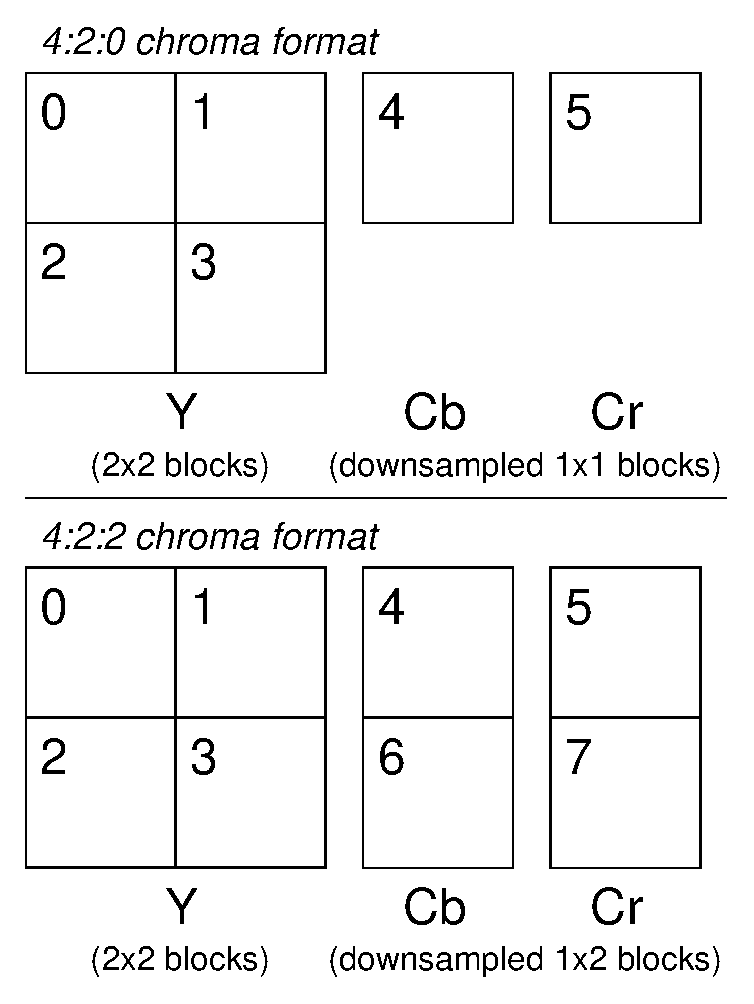
\epsfig{file=chroma_format.eps, width=2.5in}
    % \caption{4:2:0 and 4:2:2 chroma formats showing macroblock ordering}
    % \label{fig:chroma-format}
   \end{center}
  }
  \end{minipage}
  \caption{Decoding stream to handle 4:2:0 and 4:2:2 chroma
    formats. Figures on right illustrate how macroblock orderings
    differ.}
  \label{fig:chroma}
\end{figure*}

\SubSection{Motion Compensation}

An MPEG decoder accepts a bitstream as input and performs Huffman and
variable run-length decoding (VLD).  This process results in a set of
quantized, frequency-domain macroblocks and corresponding motion
vectors.  The decoder inverse quantizes (IQ) the macroblocks and then
performs an inverse DCT (IDCT) to convert the macroblocks to the
spatial domain.  For predictively coded macroblocks (e.g., P and B
pictures), the decoder performs motion compensation (MC) using the
input motion vectors to find a corresponding macroblock in a
previously decoded, stored reference picture. This reference
macroblock is added to the current macroblock to recover the original
picture data. If the current macroblock is part of an I or P picture,
then the decoder stores it for future reference.
Figure~\ref{fig:dec_block} shows the block diagram of the decode
sequence.

\begin{figure}[htbp]
\centerline{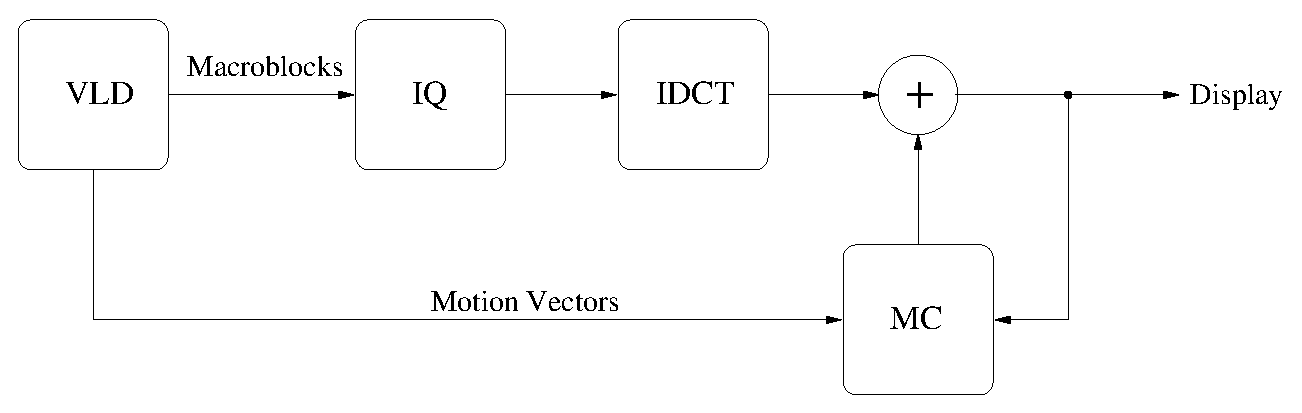
\epsfig{file=dec_block.eps,width=5in}}
\caption{Block diagram of MPEG-2 decode.}
\label{fig:dec_block}
\end{figure}

A simple strategy for parallelizing the MPEG-2 decoding can exploit
the data parallelism among macroblocks. Using this scheme, the Huffman
and run-length decoding is inherently serial, as macroblock boundaries
can only be discovered by performing the decode operation.  Once this
decode is complete, a parallel implementation can distribute
macroblocks to independent streams (using a splitjoin). Each stream
performs the inverse quantization, inverse discrete cosine transform,
and motion compensation. Furthermore, each stream locally stores
reference macroblocks for future motion compensation. Using this
strategy, the streams can execute independently with one exception.

% TODO: This is the figure showing the macroblock parallelism
% I'm not sure where it goes. - Matt
\begin{figure}
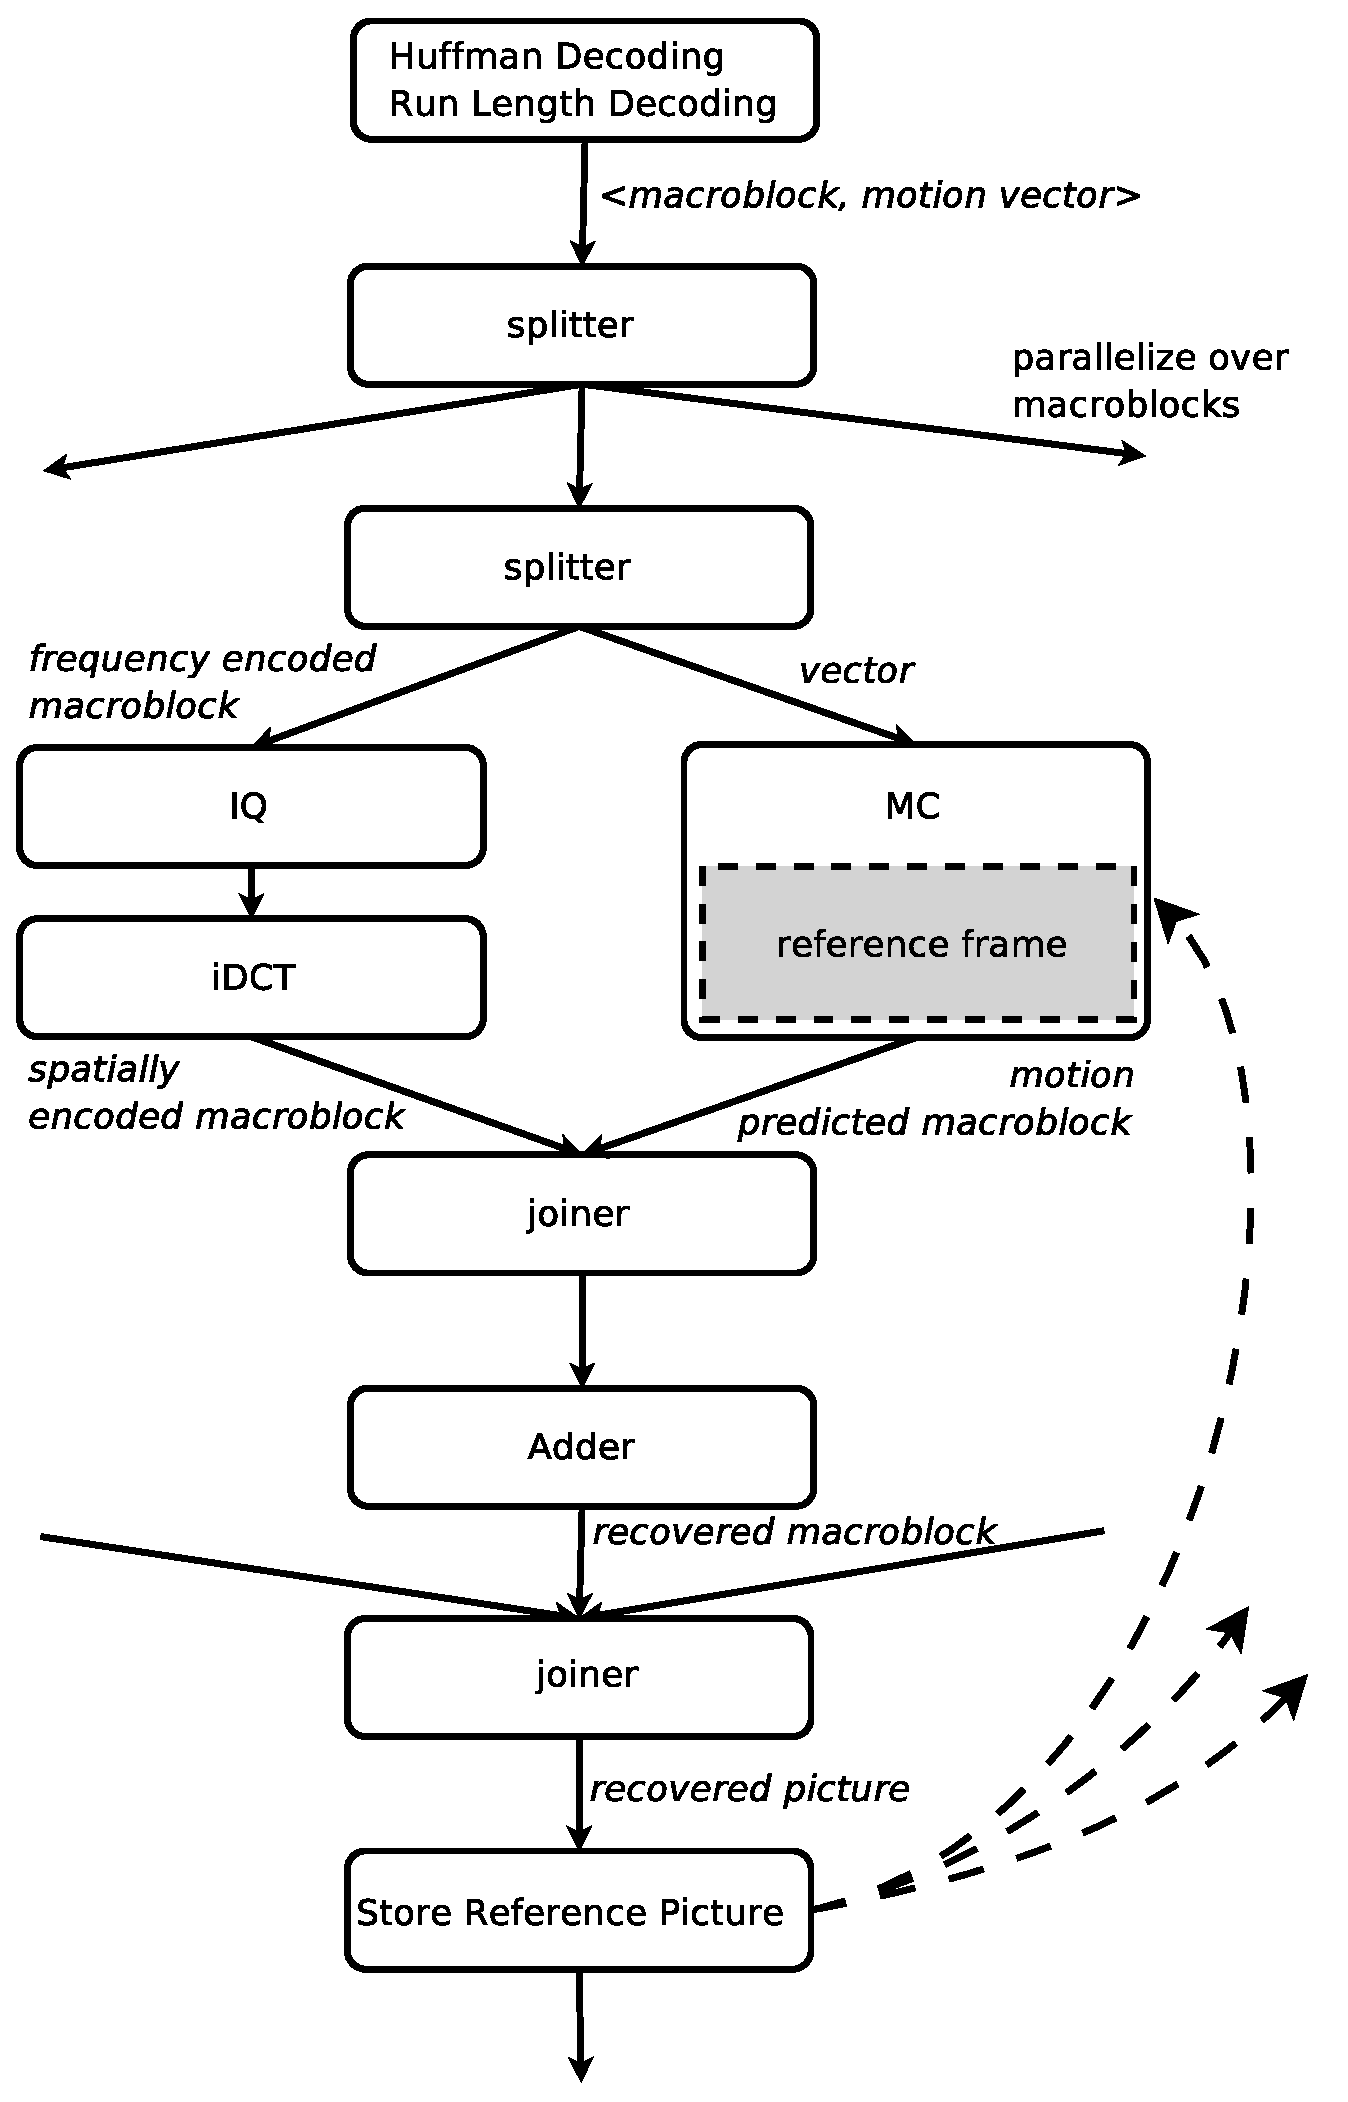
\epsfig{file=decoder_macroblock_parallelism.eps, width=3in}
% TODO: Change Matt's 2 am caption.
\caption{An MPEG-2 Decoder exploiting macroblock parallelism}
\label{decoder_macroblock_parallelism}
\end{figure}

This exception occurs when a stream is performing motion compensation
and the corresponding motion vector indicates a reference macroblock
stored in some other stream. In this case, inter-stream communication
is required to send the reference data to the requesting stream. This
situation is not uncommon, and is more prevalent for higher resolution
pictures. A simple scheme for handling this situation is for every
stream to broadcast its decoded macroblocks to all other streams. This
solution has the benefit of being conceptualy easy to understand and
implement. StreamIt allows programmers to naturally expose such
parallelism. A StreamIt pipeline that operates at macroblock
granularity is shown in Figure~\ref{fig:decoder-macroblock}. It is
worthy to note that there is a high correlation between the stream
graph, and the StreamIt syntax describing the pipeline.

%% TODO: add figure showing decoder pipeline at macroblock granularity
%% and streamit text ala Bill's beamformer/fmradio examples


